\documentclass[letterpaper,11pt]{article}
\usepackage{graphicx}
\usepackage{listings}
\usepackage[super]{nth}
\usepackage[hyphens]{url}
\usepackage{hyperref}
\usepackage{amsmath}
\usepackage[makeroom]{cancel}
\usepackage[table]{xcolor}
\usepackage{comment}
\usepackage[space]{grffile}
\usepackage{csvsimple}
\usepackage{longtable}
\usepackage{adjustbox}


\newcommand*{\srcPath}{../src}%

\lstset{
	basicstyle=\footnotesize,
	breaklines=true,
}

\begin{document}

\begin{titlepage}

\begin{center}

\Huge{Assignment 5}

\Large{CS 734:  Introduction to Information Retrieval}

\Large{Fall 2017}

\Large{Grant Atkins}

\Large Finished on \today

\end{center}

\end{titlepage}

\newpage


% =================================
% First question
% =================================
\section*{1}

\subsection*{Question}

\begin{verbatim}

\end{verbatim}

\subsection*{Answer}


%\begin{figure}[h]
%\centering
%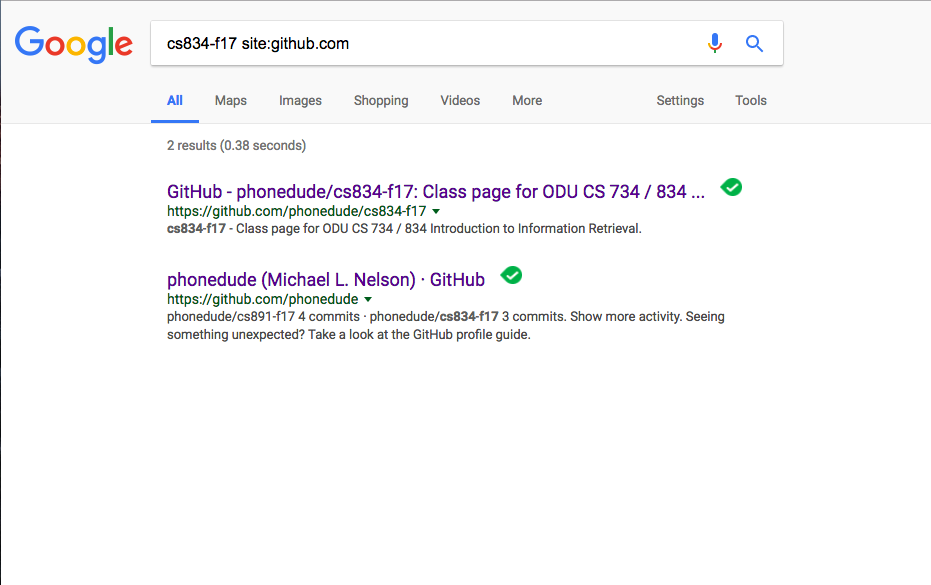
\includegraphics[scale=0.4]{sitesearch.png}
%\caption{Site search example in google}
%\label{fig:sitesearch}
%\end{figure}


\clearpage

% =================================
% Second question
% =================================

\section*{2}

\subsection*{Question}

\begin{verbatim}

\end{verbatim}

\subsection*{Answer}



\clearpage

% =================================
% 3rd question
% =================================

\section*{3}

\subsection*{Question}

\begin{verbatim}
10.6. Find two examples of document filtering systems 
on the Web. How do they build a profile for your
information need? Is the system static or adaptive?
\end{verbatim}

\subsection*{Answer}

Two examples of document filtering systems on the web are Amazon and Medium.
When buying tech accessories such as HDMI cables, keyboards, or mouses I usually go to Amazon.
Amazon keeps track of the things I browse as well as what I previously bought and attempts to make recommendations as shown in Figure \ref{fig:ama}.
This kind of filtering is an adaptive system.
If I start looking at a specific book frequently, Amazon will eventually start recommending the same book if I haven't bought it, or books that are similar to the one I viewed.

\begin{figure}[h]
\centering
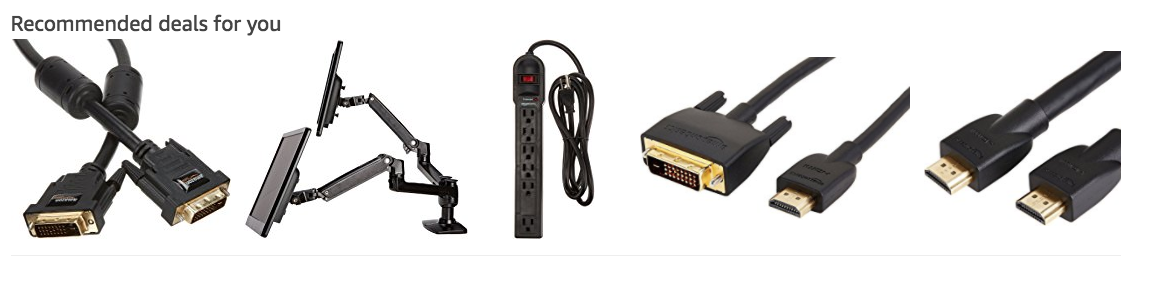
\includegraphics[scale=0.4]{amazon.png}
\caption{Amazon recommended buys}
\label{fig:ama}
\end{figure}

Another example of a document filtering system is Medium, a popular article sharing website much like blogspot.
I often enjoy reading tech related articles for machine learning, javascript, and much more on Medium.
Medium keeps track of users viewing history and then when a user visits the home page of the website it offers them lists of articles to read.
It has a ``You might like'' section where for each article it even says ``Based on your interests.''
This shows that it has filtering in place that is adaptive to my viewing history and tries to find the best trending/matching documents for my reading.
My results are shown in Figure \ref{fig:med}.

\begin{figure}[h]
\centering
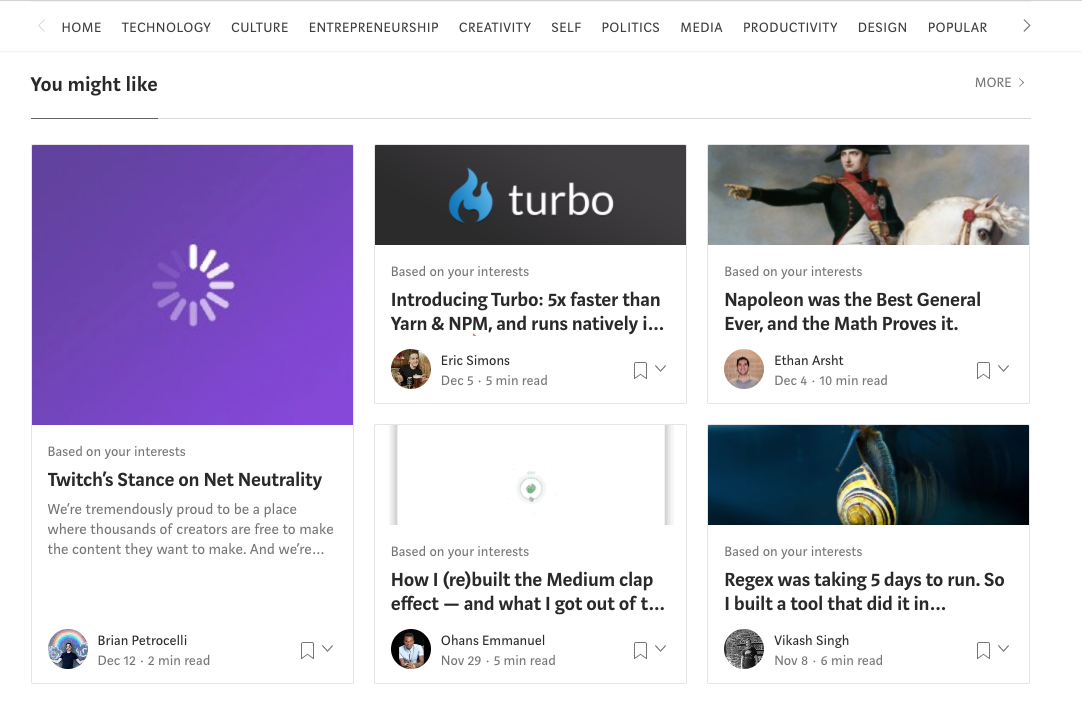
\includegraphics[scale=0.4]{medium.png}
\caption{Medium recommended reads}
\label{fig:med}
\end{figure}


% \lstinputlisting[frame=single,caption={Sitemap created from my assignment 1 (A1) directory},label=lst:sitemap_output,captionpos=b,numbers=left,showspaces=false,showstringspaces=false,basicstyle=\footnotesize]{\srcPath/data/sitemap.xml}

\clearpage

% =================================
% 4th question
% =================================

\section*{4}

\subsection*{Question}

\begin{verbatim}

\end{verbatim}

\subsection*{Answer}


\clearpage

% =================================
% 5th question
% =================================

\section*{5}

\subsection*{Question}

\begin{verbatim}
11.11. Look at a sample of images or videos that have been 
tagged by users and separate the tags into three groups: 
those you think could eventually be done automatically
by image processing and object recognition, those you think would
not be possible to derive by image processing, and spam. Also 
decide which of the tags should be most useful for queries 
related to those images. Summarize your findings.
\end{verbatim}

\subsection*{Answer}

To answer this question I decided to use Instagram to find images tagged by users.
Instagram, much like Twitter, allows for users to tag photos and posts using a \# symbol.
Its apparent that many posts on these sites bring in spam tags to get higher views or for other reasons.

For this problem I first started with a base hashtag ``\#lamborghini'' and got a lot of unexpected results as shown in Figure \ref{fig:insta_results}.
Just from the top six results, only half of the results were lamborghini model cars.
You can tell just from these results that the non lamborghini tags were probably just spam tags.

When choosing one of the images from result page, such as Figure \ref{fig:bug}, its seen that the result is actually lamborghini was a spam tag for this image.
The tags used were:

\begin{itemize}
  \item Ferrari
  \item PaganiHuaryaBC
  \item pagani
  \item supercars
  \item fast
  \item speed
  \item london
  \item omg
  \item khk
  \item harrods
  \item city
  \item nightlife
  \item lamborghini
  \item astonmartin
  \item bugatti
  \item like4like
  \item likeforfollow
  \item followforfollow
  \item follow4follow
  \item rich
  \item wealth
  \item earth
  \item lifestyle
\end{itemize}

A majority of these tags would end up in spam.
There are, however, a few of the tags that could be derived from image processing such as: 
supercars, bugatti, and city.
If a image processing is done, assuming it is accurate, then the tags that address other types of cars, such as Ferrari, PaganiHuaryaBC, lamborghini, astonmartin, and paganic, should not be grouped together with the actual descriptors of this image.
Tags that could not be taken from image processing, or rather should not, are things like wealth and earth since the first one is opinionated and earth is too broad of a topic.
Tags such as likeforlike, follow4follow, omg, speed, wealth, and a few others, are more of spam tags for this image. 
The lamborghini tag itself is also considered spam for Figure \ref{fig:bug}, as the car isn't even a lamborghini.

The tags that would be most useful for queries would be the objects actually located inside the image.
For example, bugatti is a good descriptor of the car in the image as its exactly whats in the image and it is also considered a supercar.
However, if we search for supercar then we'll get much broader search results.
So if I had to choose tags from this image, I would probably only choose bugatti if I wanted concise results.
Of course there are many tags that could be used for recommendations based off of this tag, such as rich, city, or supercar that could be recommended to users. 


\begin{figure}[h]
\centering
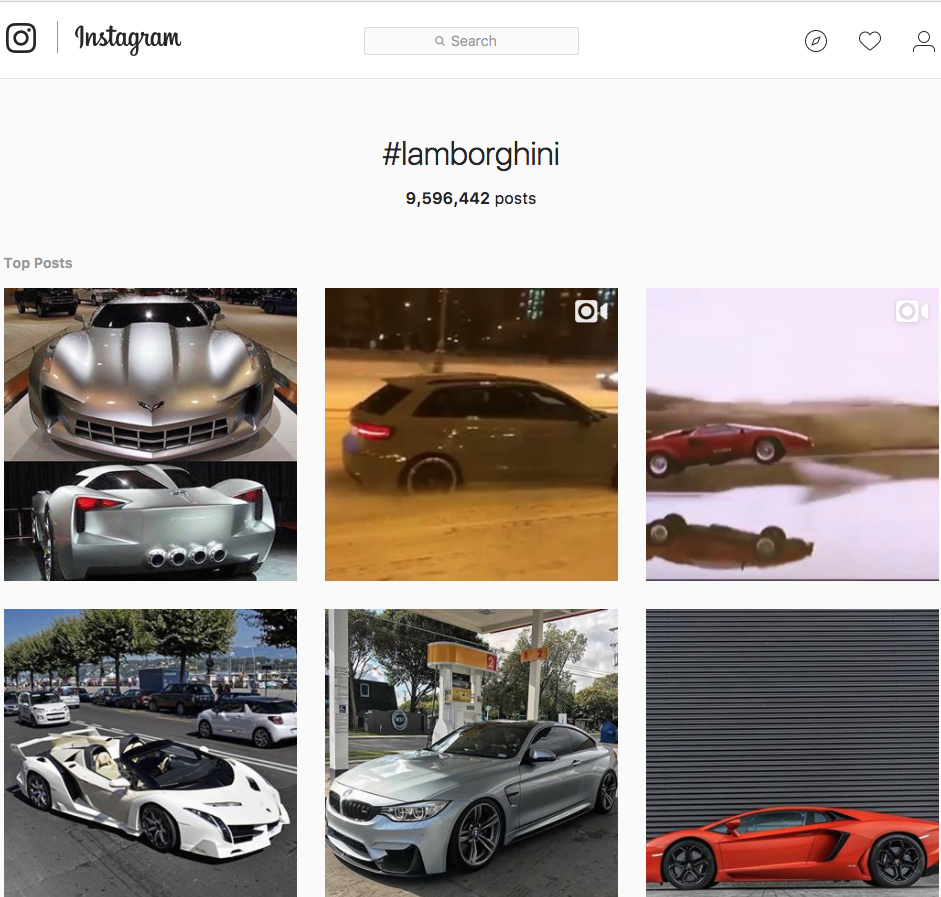
\includegraphics[scale=0.4]{insta_results.png}
\caption{Results page from Instagram}
\label{fig:insta_results}
\end{figure}

\begin{figure}[h]
\centering
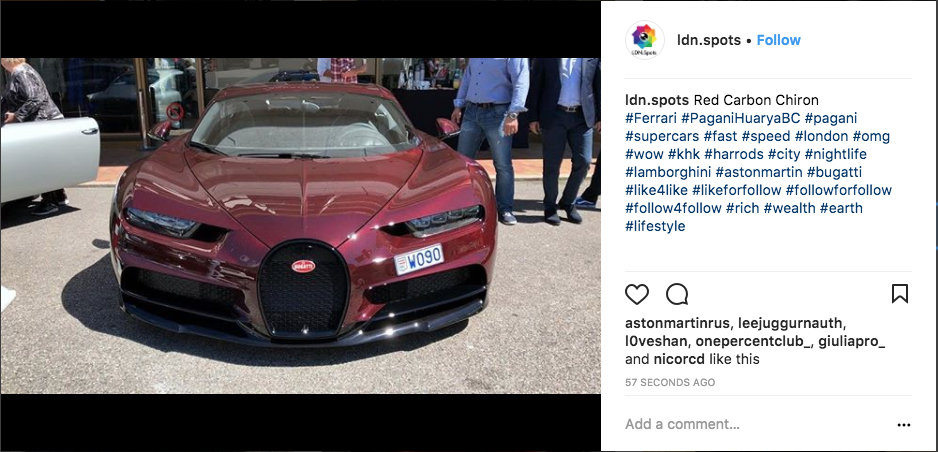
\includegraphics[scale=0.4]{multi_class.png}
\caption{Selected result from Instagram for \#lamborghini tag}
\label{fig:bug}
\end{figure}


\clearpage


\clearpage


% =================================
% Bibliography
% =================================

\begin{thebibliography}{9}
\bibitem{github}
Atkins, Grant. ``CS734 Assignment 5 Repository'' Github. N.p., 15 December 2017. Web. 15 December 2017.\url{https://github.com/grantat/cs834-f17/tree/master/assignments/A5}.
\end{thebibliography}

\end{document}
